\chapter{Bayesian Neural Networks}
A Bayesian neural network (BNN) is a probabilistic model build on the architecture of a neural network, but trained using Bayesian inference. The intent of such a model is to use the approximation capabilities of the neural networks, described in section \ref{sec:neural_network}, combined with the capability of estimating uncertainty from Bayesian inference. These uncertainty estimating capabilities comes from considering the model parameters $\boldsymbol{\theta}$ as a random variable, such that predictions are made by considering the probability distribution of $\boldsymbol{\theta}$. BNNs can therefore be viewed as a special case of ensemble learning (\cite{zhou_ensemble}) where the model ensemble is constructed by considering all possible values for $\boldsymbol{\theta}$. In practice we are not able to consider all possible values of $\boldsymbol{\theta}$ and sampling methods are used to sample different models as an approximation and there predictions are aggregated to make a single prediction.\\
\\
In section \ref{sec:bayesian_stat} we introduce two principal concepts of statistical inference; the frequentist and Bayesian paradigm and the main differences between these two paradigms. In section \ref{sec:MC_methods} we introduce the basic theory of Monte Carlo methods and in section \ref{sec:simple_BNN} we illustrate the main ideas behind Bayesian neural networks with a simple example. Since basic Monte Carlo methods are often inefficient when sampling from complex distributions we examine more sophisticated sampling methods based on Markov chains in section \ref{sec:MCMC}.
\\
\\
One of these methods is the Metropolis algorithm, which we examine in section \ref{sec:Metropolis}. Afterwards we examine the Hamiltonian Monte Carlo in section \ref{sec:HMC}. This algorithm builds on the principles of Metropolis, but explores the target distribution more efficiently. Lastly in section \ref{sec:nuts} we cover an extension of Hamiltonian Monte Carlo, that fixes possible inefficient "U-turns", called the No-U-Turn sampler. We end this chapter by briefly examining the choice of prior distributions in section \ref{sec:priors} and how one can choose the parameters for these using a distribution.





\section{Bayesian \& Frequentist Views of Learning}\label{sec:bayesian_stat}
In this section we will introduce two concepts of statistical inference. These are the Bayesian and the frequentist paradigm.
\\
\\
The ideas behind Bayesian statistics goes back to the 18th century and is named after Thomas Bayes (\cite{stigler1986history}). In Bayesian learning we consider the model parameters $\boldsymbol{\theta}$ as random and aim to learn the probability distribution of these. On the other hand the conventional frequentist methodology considers the model parameters $\boldsymbol{\theta}$ as fixed but unknown, while the point estimate $\hat{\boldsymbol{\theta}}$ is a random variable, as it is a function of the dataset, which is assumed to be random.
\\
\\
To illustrate the difference between these two approaches in more detail, we will consider an example, which involves a simple coin toss. The uncertainty of the coin showing head or tails can be expressed by the coins probability $p$ of showing heads, which is often referred to as the bias of the coin. Since the properties of the coin is not known beforehand, we do not know the exact probability of showing heads. It could be a fair coin and have the probability $p=\frac{1}{2}$ or it could be an unbalanced coin meaning that $p\neq \frac{1}{2}$.
\\
\\
A Bayesian statistician would express this uncertainty by a probability distribution over possible values of the unknown probability $p$ and would then update the distribution as more observations become known. Frequentists would find the introduction of a distribution over parameter weights as pure nonsense. The frequentist would instead flip the coin a given number of times to form a dataset, and choose some estimator, for the unknown probability $p$ which would be most consistent with the data, an obvious choice would be the relative frequency of heads in the past coin tosses. 
\\
\\
This example illustrates the main differences between these two paradigms and these differences will be highlighted in a more formal way in the subsequent sections.



\subsection{Maximum Likelihood Estimation} \label{sec:mle}
Let us now consider a dataset $\boldsymbol{X}$, with $n$ examples $\boldsymbol{x}^{(1)}, \boldsymbol{x}^{(2)},\ldots \boldsymbol{x}^{(n)}$ drawn independently from the true but unknown distribution. We let
$L(\boldsymbol{\theta}\mid \boldsymbol{X})\equiv p(\boldsymbol{X}\mid \boldsymbol{\theta})$ denote the likelihood function, where $p\lr{\boldsymbol{X}\mid\boldsymbol{\theta}}$ is a parametric family of probability distributions with parameter $\boldsymbol{\theta}$. A frequentist is, as described earlier, trying to find an estimate of the true parameter that have generated the data, we call such an estimate a point estimate and denote it by $\hat{\boldsymbol{\theta}}$ to separate it from the true parameter. A point estimate can be viewed as a function of data $\hat{\boldsymbol{\theta}}=g\lr{\boldsymbol{x}^{(1)}, \boldsymbol{x}^{(2)},\ldots \boldsymbol{x}^{(n)}}$ which is drawn from a random process meaning that $\hat{\boldsymbol{\theta}}$ is a random variable.
In most cases of frequentist inference a point estimate is found by maximizing the likelihood and is called the maximum likelihood estimate (MLE)
\begin{equation*}
\begin{split}
       \hat{\boldsymbol{\theta}}_{\text{MLE}}&=\argmax_{\boldsymbol{\theta}}{L(\boldsymbol{\theta}\mid \boldsymbol{X})}\\
        & = \argmax_{\boldsymbol{\theta}}{\prod^n_{i=1}p\lr{\boldsymbol{x}^{(i)}\mid \boldsymbol{\theta}}}
\end{split}
\end{equation*}
It is often more convenient to maximize a sum instead of a product, not only is it easier to handle sums when differentiating but it also helps stabilize the calculations numerically (\cite{Goodfellow-et-al-2016}). Thus, we take the logarithm of the likelihood function to obtain the log-likelihood function $\ell(\boldsymbol{\theta}\mid \boldsymbol{X})\equiv \log{p(\boldsymbol{X}\mid \boldsymbol{\theta})}$,
\begin{equation*}
\begin{split}
       \hat{\boldsymbol{\theta}}_{\text{MLE}}&=\argmax_{\boldsymbol{\theta}}{\ell(\boldsymbol{\theta}\mid \boldsymbol{X})}\\
        &=\argmax_{\boldsymbol{\theta}}{\sum^n_{i=1}\log{p\lr{\boldsymbol{x}^{(i)}\mid\boldsymbol{\theta}}}}
\end{split}
\end{equation*}
and since the logarithm is a monotonic-increasing function, optimizing the log-likelihood is equivalent to optimizing the likelihood. 
\\
\\
When the size of the dataset is small the MLE is often prone to overfitting and regularization methods such as penalized maximum likelihood are applied, see \cite{hastie01statisticallearning}.
\\
\\
We can generalize the maximum likelihood estimator to the case where our goal is to estimate a conditional distribution $p\lr{\boldsymbol{y}\mid \boldsymbol{X},\boldsymbol{\theta}}$, in order to predict $\boldsymbol{y}$ given $\boldsymbol{X}$ as described for supervised learning in section \ref{sec:ml_basic}. In this case the conditional maximum likelihood is given by
\begin{equation*}
    \hat{\boldsymbol{\theta}}_{\text{MLE}}=\argmax_{\boldsymbol{\theta}}L\lr{\boldsymbol{\theta}\mid \boldsymbol{y}}=\argmax_{\boldsymbol{\theta}} p(\boldsymbol{y} \mid \boldsymbol{X}, \boldsymbol{\theta})
\end{equation*}
and if assume that the targets $\boldsymbol{y}^{(1)},\ldots \boldsymbol{y}^{(n)}$ are i.i.d, we can write
\begin{equation*}
    \hat{\boldsymbol{\theta}}_{\text{MLE}}=\underset{\boldsymbol{\theta}}{\arg \max } \sum_{i=1}^{n} \log p\left(\boldsymbol{y}^{(i)} \mid \boldsymbol{x}^{(i)},\boldsymbol{\theta}\right)
\end{equation*}
The sum of squared errors, obtained by summing over all datapoints in equation \ref{eq:mse}, can be justified theoretically by the use of maximum likelihood with a Gaussian likelihood.
To see this, consider a regression model that outputs $f(\boldsymbol{X};\boldsymbol{\theta})=\boldsymbol{\theta}\boldsymbol{X}$, with real-valued targets $\boldsymbol{y}$. If we define the likelihood as the conditional distribution of $\boldsymbol{y}$ as Gaussian with mean given by the regression output $\hat{y}\equiv f(\boldsymbol{X};\boldsymbol{\theta})$ and standard deviation $\sigma$, we can write
\begin{equation*}
    L(\boldsymbol{\theta}\mid \boldsymbol{y})=\prod_{i=1}^{n} p\left(y^{(i)} \mid \boldsymbol{x}^{(i)} , \boldsymbol{\theta}\right)=\prod_i^n\frac{1}{\sqrt{2\pi\sigma}}\exp\left(-(\hat{y}^{(i)}-y^{(i)})^2/2\sigma^2\right)
\end{equation*}
Next we take the
logarithm of the likelihood function which gives us the log-likelihood function
\begin{equation*}
\begin{split}
        \ell(\boldsymbol{\theta}\mid \boldsymbol{y})&=\sum_i^n\log\frac{1}{\sqrt{2\pi\sigma}}\exp\left(-(\hat{y}^{(i)}-y^{(i)})^2/2\sigma^2\right)\\
        &=-\frac{n}{2} \log \sigma^{2}-\frac{n}{2} \log (2 \pi)-\frac{1}{2 \sigma^{2}} \sum_{i}^n\left(\hat{y}^{(i)}-y^{(i)}\right)^{2}
\end{split}
\end{equation*}
note that $-\frac{n}{2} \log \sigma^{2}-\frac{n}{2} \log (2 \pi)$ does not depend on the model parameters $\boldsymbol{\theta}$ and can therefore be omitted when maximizing. Maximizing the log-likelihood is the same as minimizing the negative log-likehood, so we can write 
\begin{equation*}
\begin{split}
        \min_{\boldsymbol{\theta}}{-\ell(\boldsymbol{\theta}\mid \boldsymbol{y})}=\frac{1}{2 \sigma^{2}} \sum_{i}^n\left(\hat{y}^{(i)}-y^{(i)}\right)^{2}
\end{split}
\end{equation*}
and since $\frac{1}{2 \sigma^{2}}$ does not depend on $\boldsymbol{\theta}$ either, we can see that minimizing the negative log-likelihood is the same as minimizing the sum of squared errors. 



\subsection{Bayesian Learning and Prediction}
A different approach than the frequentist perspective of the parameter value $\boldsymbol{\theta}$ as fixed but unknown and the point estimator $\hat{\boldsymbol{\theta}}$ as a random variable, is taken with Bayesian inference. The Bayesian paradigm considers the dataset as fixed and observable, while the true parameter $\boldsymbol{\theta}$ is unknown, and thus considered a random variable. 
\\
\\
In Bayesian statistics, we begin with defining a prior distribution $p(\boldsymbol{\theta})$ over the parameters. This prior distribution expresses our initial view on the parameters, before any data has been observed. When data becomes available, we update our prior distribution to a posterior distribution. The posterior distribution is defined by Bayes' rule
\begin{equation*}
         p(\boldsymbol{\theta}|\boldsymbol{X},\boldsymbol{y})=\frac{p(\boldsymbol{\theta})p(\boldsymbol{y}|\boldsymbol{X},\boldsymbol{\theta})}{p(\boldsymbol{y})}
\end{equation*}
and it combines the information about the data, that comes from the likelihood function $p(\boldsymbol{y}|\boldsymbol{X},\boldsymbol{\theta})$, with the prior distribution. $p(\boldsymbol{y})$ is called the model evidence and is the distribution of the observed data marginalized over the parameters $p(\boldsymbol{y})=\int p(\boldsymbol{y}\mid \boldsymbol{X}, \boldsymbol{\theta})p(\boldsymbol{\theta})d\boldsymbol{\theta}$. The model evidence is often intractable, since it requires integration over all possible values of $\boldsymbol{\theta}$, which in many applications requires integration over high-dimensional spaces. As a result, finding analytical solutions of the posterior is not possible for complex models. 
We often ignore the evidence term, as it does not depend on $\boldsymbol{\theta}$ and thus for a fixed $\boldsymbol{y}$ can be interpreted as a constant, we thus write
\begin{equation} \label{eq:posterior}
    p(\boldsymbol{\theta}|\boldsymbol{X},\boldsymbol{y})\propto p(\boldsymbol{\theta})p(\boldsymbol{y}\mid \boldsymbol{X},\boldsymbol{\theta})
\end{equation}
An important quality of the Bayesian method, is that it uses a full distribution over the parameters $\boldsymbol{\theta}$ to make predictions. Let us for example consider the case where we have observed a sample consisting of $n$ examples $\boldsymbol{X}=\boldsymbol{x}^{(1)}, \boldsymbol{x}^{(2)},\ldots, \boldsymbol{x}^{(n)}$. To predict an unobserved label $\boldsymbol{y}^{(n+1)}$ for a new example $\boldsymbol{x}^{(n+1)}$ we need the 
posterior predictive distribution, that is to integrate the model predictions by the posterior
\begin{equation} \label{eq:post_pred_distribution}
    \begin{split}
        &p\left(\boldsymbol{y}^{(n+1)} \mid \boldsymbol{x}^{(n+1)}, \lr{\boldsymbol{x}^{(1)},\boldsymbol{y}^{(1)}}, \ldots, \lr{\boldsymbol{x}^{(n)}, \boldsymbol{y}^{(n)}}\right)\\
        &=\int p\left(\boldsymbol{y}^{(n+1)} \mid \boldsymbol{x}^{(n+1)}, \boldsymbol{\theta} \right) p \lr{\boldsymbol{\theta} \mid \lr{\boldsymbol{x}^{(1)}, \boldsymbol{y}^{(1)}}, \ldots, \lr{\boldsymbol{x}^{(n)}, \boldsymbol{y}^{(n)}}} \, d \boldsymbol{\theta}
    \end{split}
\end{equation}
This is quite different from the maximum likelihood method, that uses a point estimate for $\boldsymbol{\theta}$ to make predictions on any unobserved data, the Bayesian method takes the uncertainty of estimating $\boldsymbol{\theta}$ into account when making predictions, which tends to do well in avoidance of overfitting (\cite{Goodfellow-et-al-2016}).  
\\
\\
An important difference between the Bayesian approach and MLE, lies on the contribution of a prior distribution. The prior has the effect of shifting the probability mass towards regions of the parameter space, that are preferred a priori. According to \cite{Goodfellow-et-al-2016}, the prior often expresses a preference for models that are simpler or more smooth. Critics of the Bayesian method often point their fingers at the prior distribution, and criticize it for being a subjective component that can affect the predictions of the model. According to \cite{neal2012bayesian} Bayesian methods often do a lot better than a frequentist model, when training data is limited in availability, but suffers from high computational cost when the number of training examples are large. 
\\
\\
\cite{neal2012bayesian} and \cite{mackay1991} argues that Bayesian models embodies Occam's Razor, which is the principle that we should prefer simpler models to complex ones. This principle is a component often found in machine learning since a too complex model might overfit the data. This belief is justified when model parameters are estimated by maximum likelihood, but \cite{neal2012bayesian} argues that one should not limit the complexity of Bayesian neural networks to prevent overfitting. The approach of training by minimizing loss might lead to a choice of model with increasing complexity the more data that is available. With a Bayesian approach adjusting the complexity of the model based on the amount of data available makes no sense, since a correct prior and model for 10 observations must be correct for 10.000 observations as well. One might however switch to a simple model if it seems unlikely that a complex computational expensive model will provide significant benefit. 
\\
\\
As mentioned earlier, in many practical examples, the posterior distribution is intractable and therefore must be derived in some other way. Often we will use methods such as Monte Carlo to approximate the posterior distribution. 

\subsection{Maximum a Posteriori (MAP) Estimation}
A way to avoid the computational hurdle of approximating the entire Bayesian posterior, is to use a point estimate as an approximation. Instead of turning completely to frequentist methods and use MLE, one can still benefit of the Bayesian method, by allowing the prior to influence the choice of the point estimate. One way to do this, is to use the maximum a posteriori (MAP) point estimate. The MAP estimate is obtained by maximizing the posterior distribution
\begin{equation}\label{eq: MAP}
  \begin{split}
        \hat{\boldsymbol{\theta}}_{\text{MAP}}&=\argmax_{\boldsymbol{\theta}}{p(\boldsymbol{\theta}\mid \boldsymbol{X},\boldsymbol{y}})=\argmax_{\boldsymbol{\theta}}{p(\boldsymbol{y}\mid \boldsymbol{X},\boldsymbol{\theta}}) p(\boldsymbol{\theta})\\
        &=\argmax_{\boldsymbol{\theta}}{\log p(\boldsymbol{y}\mid \boldsymbol{X},\boldsymbol{\theta}})+ \log p(\boldsymbol{\theta})
  \end{split}
\end{equation}
note that the evidence term has been omitted, since it does not depend on the parameter $\boldsymbol{\theta}$ and thus vanishes under maximization anyway. The bottom part of equation \ref{eq: MAP} can be recognized as an equation consisting of the standard log-likelihood term plus a log-prior term. \\
\\
As an example, consider a model with a Gaussian prior placed on the regression weights $\boldsymbol{\theta}$. If we specifically choose the prior to be given by $\mathcal{N}\left(\boldsymbol{\theta},0,\frac{1}{\alpha}\boldsymbol{I}^2\right)$, then the log-prior term in equation \ref{eq: MAP} is proportional to the L2 norm introduced in \ref{eq:L2_reg}, plus a term that does not depend on $\boldsymbol{\theta}$.
Note also that the MAP estimate is the same as the MLE, when choosing a uniform prior, since the $p(\boldsymbol{\theta})$ becomes a constant function in equation \ref{eq: MAP} and consequently we can ignore it when maximizing the expression. Compared to MLE, MAP estimation has the advantage that it can benefit from the information in the prior that cannot be found in the dataset. According to \cite{Goodfellow-et-al-2016} this additional information, gained from the choice of prior, can reduce the variance in the MAP point estimate in direct comparison with MLE estimate, but this advantage has a price of an increased bias.
\\
\\
MAP is closely related to Bayes optimal estimation, instead of finding the most probable hypothesis (set of parameters), it aims at finding the most probable label for a new example. The Bayes optimal estimation is done by predicting the $\boldsymbol{y}^{(n+1)}$, which maximizes the posterior predictive distribution in equation \ref{eq:post_pred_distribution}. We do not pursue the idea of Bayes optimal estimation, as we aim to minimize a loss function which is not always equivalent to predicting the most probable label. In this way we preserve the idea that the loss function dictates how much the algorithm should care about making certain predictions as explained in \ref{sec:loss_func}.
\\
\\
An obvious disadvantage from using MAP estimation, is that it discards the information contained in the distribution. It is estimating distributions that make Bayesian methods attractive, especially if one wants to evaluate the uncertainty of the parameters. As we value access to this distribution higher than faster computational time we will not pursue MAP estimation any further.

\section{Monte Carlo Methods}\label{sec:MC_methods}
One way of approximating intractable integrals, like the posterior predictive distribution in equation \ref{eq:post_pred_distribution}, is to use Monte Carlo methods. The idea behind Monte Carlo methods is to view the integral as an expectation of some random variable with respect to a probability distribution $p(\cdot)$. In the case of BNNs our random variable is the model parameters $\boldsymbol{\theta}$, and we can write the posterior predictive distribution as
\begin{equation}
    \begin{split}
        &p\left(\boldsymbol{y}^{(n+1)} \mid \boldsymbol{x}^{(n+1)}, \lr{\boldsymbol{x}^{(1)},\boldsymbol{y}^{(1)}}, \ldots, \lr{\boldsymbol{x}^{(n)}, \boldsymbol{y}^{(n)}}\right)\\
        &=\int p\left(\boldsymbol{y}^{(n+1)} \mid \boldsymbol{x}^{(n+1)}, \boldsymbol{\theta}\right) p \lr{\boldsymbol{\theta} \mid \lr{\boldsymbol{x}^{(1)}, \boldsymbol{y}^{(1)}}, \ldots, \lr{\boldsymbol{x}^{(n)}, \boldsymbol{y}^{(n)}}} \, d \boldsymbol{\theta}\\
        &=\int f\lr{\boldsymbol{\theta}}\hat{p}\lr{\boldsymbol{\theta}} d\boldsymbol{\theta}
    \end{split}
\end{equation}
where we use a simpler notation of $\hat{p}\lr{\boldsymbol{\theta}}$ to denote the posterior distribution. Such an integral can be interpreted as an expectation taking under the probability distribution $\hat{p}(\boldsymbol{\theta})$ 
\begin{equation*}
    s=\int f(\boldsymbol{\theta})\hat{p}(\boldsymbol{\theta})  d \boldsymbol{\theta}=\mathbb{E}_{\hat{p}}[f(\boldsymbol{\theta})]
\end{equation*}
Now in order to approximate $s$ we can draw samples from the distribution $\hat{p}(\boldsymbol{\theta}) $ and approximate the expected value by the empirical average. If we draw $n$ samples $\boldsymbol{\theta}\sim \hat{p}(\boldsymbol{\theta})$ we can approximate $s$ by $\hat{s}_n$
\begin{equation}\label{eq:empirical_mean_MC}
        \hat{s}_{n}=\frac{1}{n} \sum_{i=1}^{n} f\left(\boldsymbol{\theta}^{(i)}\right)
\end{equation}
This implies the simplest situation, where it is possible to simulate directly from the probability distribution, which is often not possible.
\\
\\
We can justify this approximation theoretically, by noticing that $\hat{s}_n$ is an unbiased estimator of $s$
\begin{equation*}
    \mathbb{E}_{\hat{p}}\left[\hat{s}_{n}\right]=\frac{1}{n} \sum_{i=1}^{n} \mathbb{E}_{\hat{p}}\left[f\left(\boldsymbol{\theta}^{(i)}\right)\right]=\frac{1}{n} \sum_{i=1}^{n} s=s
\end{equation*}
additionally the law of large numbers, states that if the samples $\boldsymbol{\theta}^{(i)}$ are independent and identical distributed (i.i.d), the empirical average converges to the true expectation almost surely
\begin{equation*}
    \lim _{n \rightarrow \infty} \hat{s}_{n}=s
\end{equation*}
this only holds if the variance of the individual terms $\operatorname{Var}[f\lr{\boldsymbol{\theta}^{(i)}}]$ is bounded. To see this, we note that $\operatorname{Var}[\hat{s}_n]$ converges to zero as n goes to infinity, if and only if $\operatorname{Var}[f\lr{\boldsymbol{\theta}}]<\infty$
\begin{equation*}
    \begin{split}
\operatorname{Var}\left[\hat{s}_{n}\right] &=\operatorname{Var}\left[\frac{1}{n} \sum_{i=1}^{n} f(\boldsymbol{\theta}^{(i)})]\right] \\ &=\frac{1}{n^{2}} \sum_{i=1}^{n} \operatorname{Var}[f(\boldsymbol{\theta}^{(i)})]
=\frac{\operatorname{Var}[f(\boldsymbol{\theta})]}{n}
\end{split}
\end{equation*}
Further the central limit theorem states that, if $\mathbb{E}_{\hat{p}}[f(\boldsymbol{\theta})]=s$ and $\operatorname{Var}[f(\boldsymbol{\theta})]<\infty$ then
\begin{equation*}
    \frac{\hat{s}_{n}-s}{\sqrt{\operatorname{Var}[f(\boldsymbol{\theta})] / n}} \sim \mathcal{N}(0,1)
\end{equation*}
which is equivalent to
\begin{equation*}
    \hat{s}_n\sim \mathcal{N}\left(s,\frac{\operatorname{Var}[f(\boldsymbol{\theta})]}{n}\right)
\end{equation*}
Which gives us a way of estimating confidence intervals around the estimate $\hat{s}$. \\
\\
When it is infeasible or not possible to make simulations of $\boldsymbol{\theta}$ directly, Markov chain Monte Carlo methods can be used. such methods simulate from a target distribution by running a Markov chain, that eventually will converge to target distribution. Markov chain Monte Carlo methods will be examined more thoroughly in section \ref{sec:MCMC}.



\section{A Simple Bayesian Neural Network} \label{sec:simple_BNN}
A simple example, inspired by \cite{neal2012bayesian}, will illustrate the general concept of Bayesian learning for neural networks and the inefficiency of brute force methods of sampling. Figure \ref{fig:simple_BNN} shows six BNNs whose weights and biases were drawn from independent standard normal prior distributions except output weights, which had a standard deviation of $\frac{1}{\sqrt{16}}$. The networks performs regression on six data points. 
\\
\\
The six networks was chosen from a larger pool of $10^5$ networks with weights and biases sampled from identical prior distributions. The likelihood was computed for each of these networks and scaled so that the largest likelihood was 1. The networks were then accepted with the probability of this scaled likelihood for which only six was accepted. This approach resembles rejection sampling and embodies the posterior from equation \ref{eq:posterior} by making the prior control the generation of candidate networks and the likelihood control which of these candidates are rejected.
We follow the suggestion of \cite{neal2012bayesian} to model regression tasks with a conditional distribution for the real valued targets $\boldsymbol{y}_k$, from $k$ neural networks with outputs $f_k(\boldsymbol{x})$, defined by a Gaussian distribution
\begin{equation}\label{eq:regr_taget_distribution}
    p(\boldsymbol{y} \mid \boldsymbol{x}) = \prod_k \frac{1}{\sqrt{2 \pi} \sigma_k} \exp{- \frac{\lr{f_k(\boldsymbol{x}) - y_k}^2}{2 \sigma_k^2}}
\end{equation}
with mean $f_k(\boldsymbol{x})$ and standard deviation $\sigma_k$ as a hyperparameter, which we choose to be $\sigma_k = 0.1$ for all $k$.
\\
\\
According to \cite{neal2012bayesian} the optimal way to predict the target associated with various new examples, assuming we want to minimize the expected squared error, is to predict the mean of the predictive distribution in equation \ref{eq:post_pred_distribution}. For a regression model defined by equation \ref{eq:regr_taget_distribution} this is equal to predicting 
\begin{equation*}
    \hat{\boldsymbol{y}}^{(n+1)} = \int f\lr{\boldsymbol{x}^{(n+1)}, \boldsymbol{\theta}} p\lr{\boldsymbol{\theta} \mid \lr{\boldsymbol{x}^{(1)}, \boldsymbol{y}^{(1)}}, \dots, \lr{\boldsymbol{x}^{(n+1)}, \boldsymbol{y}^{(n+1)}}} \, d \boldsymbol{\theta}
\end{equation*}
As we do not know this distribution, we resort to a Monte Carlo approximation by averaging over the outputs from the six neural networks, obtained by sampling parameters from the posterior. The average is shown in figure \ref{fig:simple_BNN} by the solid line. But Bayesian inference can do more than a single-valued guess. By examining the function we can also see the uncertainty of the guesses, for example how rapidly uncertainty increases beyond the region of the data points. 
\\
\\
This illustrates some of the benefits of using Bayesian inference for neural networks, but what remains is the downside of computational time. Generating $10^5$ samples to get six draws from the posterior is not very efficient and this only becomes more infeasible as the number of data points increase. 
\begin{figure}
    \centering
    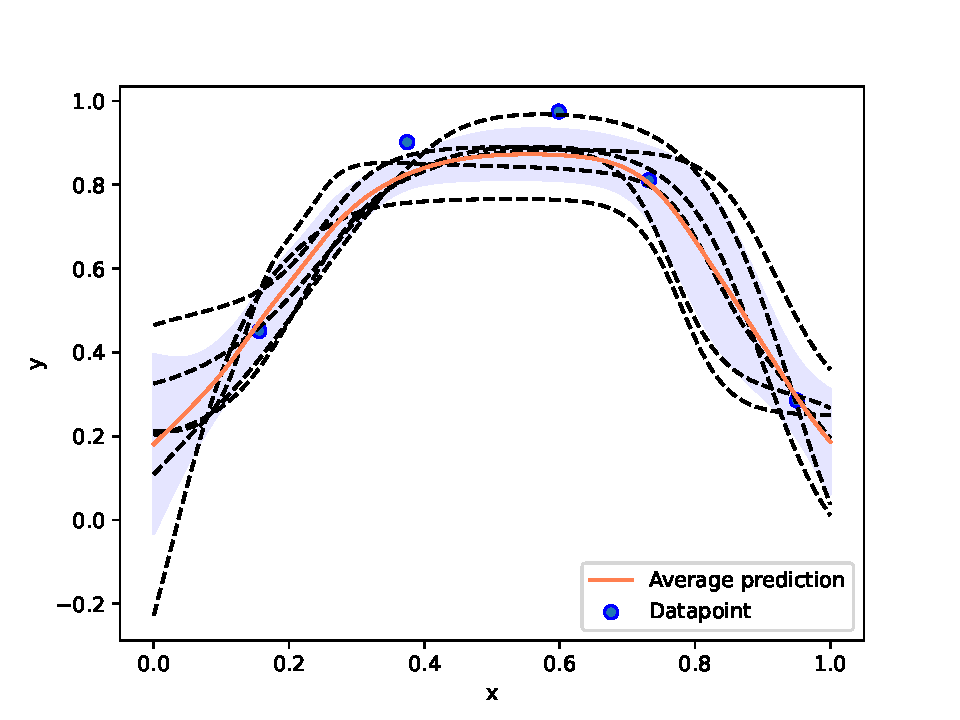
\includegraphics[width=\textwidth,height=\textheight,keepaspectratio]{pics/figure_simple_BNN.pdf}
    \caption{Sampled neural networks from a posterior predictive distribution that is based on a Gaussian prior and a Gaussian likelihood on the six data points. The average prediction of the networks are plotted along with a filled area defined by the average plus minus the standard deviation of the network predictions to represent uncertainty. The Python code for implementing this Bayesian neural network and the production of this figure can be seen in appendix \ref{app:simple_BNN}}
    \label{fig:simple_BNN}
\end{figure}
\clearpage
\section{Markov Chain Monte Carlo}\label{sec:MCMC}
 As mentioned in section \ref{sec:bayesian_stat} the posterior distribution is often intractable and we might need simulation based methods to find a feasible solution. We want to be able to calculate posterior summaries like $\mathbb{E}_{\hat{p}}\left[f(\boldsymbol{\theta})\right]$ where $f(\boldsymbol{\theta})$ is some function over the parameters and the expectation is taken under the posterior distribution. Such an expectation is straightforward to approximate using the simple Monte Carlo method, described in section \ref{sec:MC_methods}, when dealing with nice and low dimensional distributions. Other methods like importance sampling has often been proposed in the litterateur for simple problems, but rarely for high-dimensional problems as we often face with neural networks.
 \\
 \\
The simple example in section \ref{sec:simple_BNN} illustrated that brute force methods are also not very useful in complex models like BNNs and we are instead motivated to use a collection of more sophisticated methods. This thesis will mainly pursue this motivation by exploring the Markov chain Monte Carlo (MCMC) methods. The main idea is to simulate a Markov chain, which has the posterior distribution as its stationary distribution. We will initially give a concise explanation of the fundamentals of Markov chains in section \ref{sec:basic_mc} and follow this by exploring the most popular MCMC algorithms for sampling in BNNs.
 
 
\subsection{Markov Chains}\label{sec:basic_mc}

A stochastic process is a set of random variables that are defined over some probability space $\left\{X^{(t)} \right\}_{t\in T}$, where $T\subseteq \mathbb{R}$ is the indexation and may be interpreted as a time index. In the context of machine learning, the set $T$ can be interpreted as the iterations of a simulation scheme. In stochastic simulation we typically have that $T=\mathbb{N}$ and we can write the stochastic process as $\left\{X^{(n)}\right\}_{n\geq 0}$, where $n$ reminds us that we have a discrete index set. Throughout this thesis we will only consider discrete time stochastic processes, since this is found to be most relevant when discussing stochastic simulation. \\
A stochastic process is defined over a space of possible values called the state space $\mathbb{S}$ and will in most applications be either integers or real values. 
\\
\\
With the objective of modelling BNNs, we want to sample model parameters from the posterior distribution. These samples will then be used to make predictions for unseen data by approximating the posterior predictive distribution from equation \ref{eq:post_pred_distribution} via Monte Carlo integration. In order to do this using MCMC we will consider the stochastic process $\{\boldsymbol{\theta}^{(n)}\}_{n\geq 0}$. To make the description of MCMC methods more general in the next sections, we will denote the distribution we aim to sample from the target distribution and denote it $\hat{p}(\cdot)$. The target distribution in the case of BNNs is the posterior of the weights such that $\hat{p}(\boldsymbol{\theta})\equiv p(\boldsymbol{\theta}\mid \boldsymbol{X},\boldsymbol{y})$.
\\
\\
Using Markov chain Monte Carlo we aim to sample from a stochastic process satisfying the Markov property. Such a process is defined by being dependant only on the previous state of the process and a set of transitional probabilities, or densities for a infinite state space, and is called a Markov chain. The Markov chain is defined by an initial distribution for the first state of the chain $\boldsymbol{\theta}^{(0)}$, and a transition density for the next states in the system. We write the transition density from transitioning from state $\boldsymbol{\theta}^{(n-1)}$ to another state $\boldsymbol{\theta}^{(n)}$ as $T(\boldsymbol{\theta}^{(n)}\mid \boldsymbol{\theta}^{(n-1)})$. \\
\\
When sampling from the Markov chain we want to make sure that samples are actually coming from the desired distribution $\hat{p}(\boldsymbol{\theta})$ no matter the initial distribution. To ensure this we must generate a Markov chain that has our desired distribution  $\hat{p}\lr{\boldsymbol{\theta}}$ as a stationary distribution. That is if $\boldsymbol{\theta}^{(n-1)}$ has distribution $\hat{p}(\cdot)$, then  $\boldsymbol{\theta}^{(n)}$ will have the same distribution, and this will hold for all future states of the chain. The property of a Markov chain having a stationary distribution is called the invariance property and is defined by
\begin{equation*}
    \pi(\boldsymbol{\theta}^{(n)})=\int T(\boldsymbol{\theta}^{(n)}\mid \boldsymbol{\theta}) \pi(\boldsymbol{\theta})d\boldsymbol{\theta}
\end{equation*}
A sufficient, but not necessary condition, that ensures that a particular $\hat{p}(\boldsymbol{\theta})$ is stationary distribution is the detailed balance condition. The condition states if we let $T(\cdot,\cdot)$ be a transition density, which satisfies the following condition 
$$T(\boldsymbol{\theta}^{(n-1)}, \boldsymbol{\theta}^{(n)}) \hat{p}(\boldsymbol{\theta}^{(n)})= T(\boldsymbol{\theta}^{(n)}, \boldsymbol{\theta}^{(n-1)})\hat{p}(\boldsymbol{\theta}^{(n-1)})$$
then $\hat{p}(\cdot)$ is a stationary distribution of the Markov chain associated with the transition density $T(\cdot,\cdot)$. This property however only ensures that $\hat{p}\lr{\boldsymbol{\theta}}$ is stationary distribution but not that it is the only one, meaning that our Markov chain can end up sampling from the wrong distribution, even though it satisfies the detailed balance condition.
\\
\\
To guarantee that we sample from $\hat{p} \lr{\boldsymbol{\theta}}$ we need to ensure that the Markov chain has only this distribution as a stationary distribution. A Markov chain which has a unique stationary distribution, from which it converges to, from any initial state is called an ergodic Markov chain (see e.g \cite{turkman2019computational}). For a Markov chain on a finite state space to be ergodic, it has to be irreducible and aperiodic. The same goes for a Markov chain on a infinite state space, but a slightly stronger condition called Harris recurrence is needed, see \cite{gamerman2006markov}.                                   
\\
\\
Often we discard or burn some of the initial states, since these may not be representative of the desired distribution, as the chain might not have reached the stationary distribution yet. These discarded steps are part of what is called the  burn-in period of the Markov chain. When the chain has reached the stationary distribution, it is possible to draw as many identical distributed samples as we wish for, but one should note that any successive samples will be highly correlated with each other and therefore not necessarily a good representative for the target distribution. \cite{Goodfellow-et-al-2016} suggest a way to mitigate this problem, by only returning every $n$ successive sample. Because of both the burn-in period and the time required for the chain to return uncorrelated samples MCMCs are often computational expensive. \\
\\
In order to produce truly independent samples, \cite{Goodfellow-et-al-2016} suggest to run multiple Markov chains in parallel. They also mention that practitioners often chooses the number of chains to run in parallel, similar to the number of examples in a mini-batch and then draw the samples needed from this set of Markov chains. 


\subsection{The Metropolis algorithm} \label{sec:Metropolis}
The Metropolis algorithm is a MCMC method, which is used to sample from a distribution. 
The Metropolis algorithm was originally introduced by \cite{Metropolis1953} and was developed to simulate the states for a system of molecules. This was later further developed by \cite{hastings70}, so that the algorithm could now simulate from a general distribution and not just a symmetric one, as it was previously based on. The Metropolis algorithm is an attractive MCMC method due to its versatility and simplicity.\\
\\
The algorithm considers a target distribution $\hat{p}(\boldsymbol{\theta})$ and a proposal distribution $q(\boldsymbol{\theta})$. The algorithm generates a Markov chain, by starting the chain at some arbitrarily point generated from the proposal distribution $\boldsymbol{\theta}^{(0)}\sim q(\boldsymbol{\theta})$ and then proposing a candidate state for the next state in the chain $\boldsymbol{\theta}^{\text{\text{cand}}}$, where this candidate state is drawn from the conditional distribution on the previous state $\boldsymbol{\theta}^{\text{\text{cand}}}\sim q(\boldsymbol{\theta}^{(n+1)}\mid\boldsymbol{\theta}^{(n)})$. The next step is to decide whether or not to reject this new state based on the relative density to the old state. If the relative density is larger than one, we accept the new state, if the relative density is less than one, we accept the new state with probability $\frac{\hat{p}(\boldsymbol{\theta}^{\text{\text{cand}}})}{\hat{p}(\boldsymbol{\theta}^{(n)})}$. In this context the Metropolis algorithm imposes the symmetry condition of on the proposal distribution, so that
\begin{equation*}
    q(\boldsymbol{\theta}^{(n)}\mid \boldsymbol{\theta}^{(n-1)})=q(\boldsymbol{\theta}^{(n-1)}\mid \boldsymbol{\theta}^{(n)})
\end{equation*}
A pseudocode version of the Metropolis algorithm can be seen in algorithm \ref{algo_2}.
% Metropolis Algorithm
\begin{algorithm}\label{algo_2}

\SetAlgoLined
\KwInput{A proposal distribution $q$}
\KwOutput{A set of parameters $\boldsymbol{\theta^{(n)}}$ for $n = 1, \dots, N$}
initialize $\boldsymbol{\theta}^{(0)}\sim q(\boldsymbol{\theta})$;

\For{$n=1,2,\ldots, N$}{
Propose: $\boldsymbol{\theta}^{\text{\text{cand}}} \sim q\left(\boldsymbol{\theta}^{(n)} \mid \boldsymbol{\theta}^{(n-1)}\right)$

Acceptance Probability:

$ \alpha\left(\boldsymbol{\theta}^{\text{\text{cand}}} \mid \boldsymbol{\theta}^{(n-1)}\right)=\min \left\{1, \frac{\hat{p}\left(\boldsymbol{\theta}^{\text{\text{cand}}}\right)}{ \hat{p}\left(\boldsymbol{\theta}^{(n-1)}\right)}\right\} $

$u \sim  \text { Uniform }(0,1)
$

  \uIf{$u<\alpha$}{
    Accept the proposal: $\boldsymbol{\theta}^{(n)} \leftarrow \boldsymbol{\theta}^{\text{\text{cand}}}$\;
  }
  \Else{
    Reject the proposal: $\boldsymbol{\theta}^{(n)} \leftarrow \boldsymbol{\theta}^{(n-1)}$ \;
  }
    }
\caption{Metropolis algorithm}
\end{algorithm}
One apparent problem is that due to the evidence term we can not calculate the posterior exactly, which is our target distribution $\hat{p}\lr{\boldsymbol{\theta}}$, so we can not directly calculate $\frac{\hat{p}(\boldsymbol{\theta}^{(n)})}{\hat{p}\left(\boldsymbol{\theta}^{(n-1)}\right)}$. 
But a nice property of Metropolis acceptance probability is that we only need a function that is proportional to the posterior, as any constant of proportionality will cancel out in the calculation of the acceptance probability. As the evidence term can be interpreted as a constant of proportionality, it will cancel out and we can instead use equation \ref{eq:posterior} and calculate the ratio of the likelihood times the prior, which we are often able to.   
\\
\\
To show that the Metropolis algorithm is in fact sampling from the target distribution, we must show that the Markov chain converges to a stationary distribution which is our target distribution. If we assume that the Markov Chain is ergodic we can do this by showing that the metropolis satisfies the detailed balanced condition explained in section \ref{sec:MCMC}.\\
\\
For $\boldsymbol{\theta}^{(n)}\neq \boldsymbol{\theta}^{(n-1)}$ the Metropolis algorithm has the following transitions densities,
\begin{equation*}
    T\left(\boldsymbol{\theta}^{(n)} \mid \boldsymbol{\theta}^{(n-1)}\right)=q\left(\boldsymbol{\theta}^{(n)} \mid \boldsymbol{\theta}^{(n-1)}\right) \min \left(1, \frac{\hat{p}\left(\boldsymbol{\theta}^{(n)}\right)}{ \hat{p}(\boldsymbol{\theta}^{(n-1)})}\right)
\end{equation*}
We can show that this satisfies the detailed balanced condition by
\begin{equation*}
\begin{aligned}
T\left(\boldsymbol{\theta}^{(n)} \mid \boldsymbol{\theta}^{(n-1)}\right) \hat{p}(\boldsymbol{\theta}^{(n-1)}) &=q\left(\boldsymbol{\theta}^{(n)} \mid \boldsymbol{\theta}^{(n-1)}\right) \min \left(1,\frac{ \hat{p}\left(\boldsymbol{\theta}^{(n)}\right) }{ \hat{p}(\boldsymbol{\theta}^{(n-1)})}\right) \hat{p}(\boldsymbol{\theta}^{(n-1)}) \\
&=q\left(\boldsymbol{\theta}^{(n)} \mid \boldsymbol{\theta}^{(n-1)}\right) \min \left(\hat{p}(\boldsymbol{\theta}^{(n-1)}), \hat{p}\left(\boldsymbol{\theta}^{(n)}\right)\right) \\
&=q\left(\boldsymbol{\theta}^{(n-1)} \mid \boldsymbol{\theta}^{(n)}\right) \min \left(\hat{p}\left(\boldsymbol{\theta}^{(n-1)}\right), \hat{p}(\boldsymbol{\theta}^{(n-1)})\right) \\
&=q\left(\boldsymbol{\theta}^{(n-1)} \mid \boldsymbol{\theta}^{(n)}\right) \min \left(1, \frac{\hat{p}(\boldsymbol{\theta}^{(n-1)}) }{ \hat{p}\left(\boldsymbol{\theta}^{(n)}\right)}\right) \hat{p}\left(\boldsymbol{\theta}^{(n)}\right) \\
&=T\left(\boldsymbol{\theta}^{(n-1)} \mid \boldsymbol{\theta}^{(n)}\right) \hat{p}\left(\boldsymbol{\theta}^{(n)}\right)
\end{aligned}
\end{equation*}
This shows that the transitions proposed by the algorithm leaves the target distribution $\hat{p}(\boldsymbol{\theta})$ invariant and therefore samples produced by this Markov chain all has the same stationary distribution $\hat{p}(\boldsymbol{\theta})$, provided that the Markov chain is ergodic. However according to \cite{neal2012bayesian} the Metropolis algorithm will not always produce an ergodic Markov chain and that this depends on the details of the target distribution and proposal distribution. If the produced Markov chain is not ergodic we might end up sampling from a stationary distribution that is not our target distribution.
\\
\\
There are many possible choices for the proposal distribution. \cite{neal2012bayesian} mentions that a simple choice could be a Gaussian centered on $\boldsymbol{\theta}^{(n)}$ with standard deviation chosen so that the acceptance probability of the candidate state is reasonably high, since a very low acceptance ratio is usually unwanted, as many rejections means that we are inefficiently wasting computation time. He also notes that when sampling from high-dimensional and complex distributions, which is often the case with posteriors in BNNs, the standard deviation of such a proposal distribution will often have to be small compared to the extent of the target distribution, as large changes almost certainly will lead to a region of low probability. This will result in highly dependant states and many steps will be needed to arrive at distant points in the distribution. As suggested in section \ref{sec:basic_mc} one way of coping with this problem is to throw away some of the samples or run multiple chains in parallel. \\
\\
\cite{neal2012bayesian} further mentions that this problem with Metropolis is made worse due to its movements taking the inefficient form of a random walk instead of a systematic path, as can be seen in the illustration of a sampling with Metropolis in figure \ref{fig:MH_sampling}. This inefficient movement yields slower convergence to the target distribution. This drawback, will be even more prominent in higher dimension and for more complex target distributions according to \cite{gelmanbda04}. \\
\\
A more generalized version of the algorithm is the one introduced by \cite{hastings70}, which allows for non-symmetric proposal distributions $q(\boldsymbol{\theta}^{(n)}\mid \boldsymbol{\theta}^{(n-1)}) \neq q(\boldsymbol{\theta}^{(n-1)}\mid \boldsymbol{\theta}^{(n)})$. To correct for this asymmetry in the proposal distribution, the acceptance ratio is replaced by
\begin{equation}\label{eq: hasti_pasti}
\alpha\left(\boldsymbol{\theta}^{c a n d} \mid \boldsymbol{\theta}^{(n-1)}\right)=\min \left\{1, \frac{q\left(\boldsymbol{\theta}^{(n-1)} \mid \boldsymbol{\theta}^{c a n d}\right) \hat{p}\left(\boldsymbol{\theta}^{c a n d}\right)}{q\left(\boldsymbol{\theta}^{c a n d} \mid \boldsymbol{\theta}^{(n-1)}\right) \hat{p}\left(\boldsymbol{\theta}^{(n-1)}\right)}\right\} 
\end{equation}
One should note that the Metropolis algorithm is an instance of the generalized version, since equation \ref{eq: hasti_pasti} is identical to the acceptance ratio in the original algorithm when allowance for a symmetric distribution. \\
\\
The introduction of an asymmetric proposal distribution, is often useful when we want to increase the speed of the random walk generated by the Metropolis algorithm. However, this is often not sufficient for complicated models with high-dimensional target distributions as we face with Bayesian neural networks, see \cite{gelmanbda04}.
\begin{figure}
    \centering
    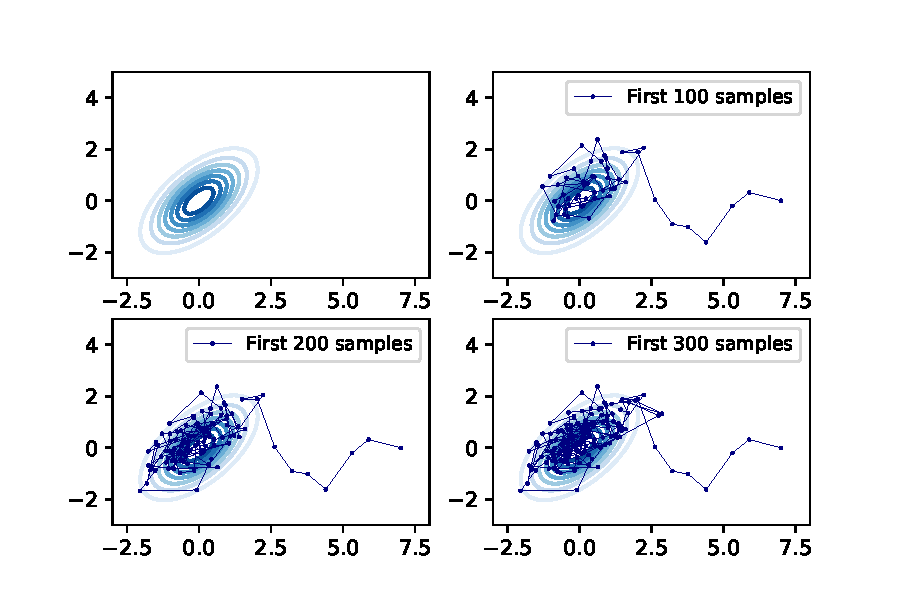
\includegraphics[width=\textwidth, height=\textheight, keepaspectratio]{pics/mh_randomWalk_behavior.pdf}
    \caption{Illustration of the convergence to a target distribution with 300 samples from the Metropolis algorithm. The target distribution is a bivariate Gaussian with mean 
        $\boldsymbol{\mu}= \begin{bmatrix}
            0 & 0
            \end{bmatrix}$ and covariance matrix
            $\boldsymbol{\Sigma}= 
            \begin{bmatrix}
                1 & 0.6\\
                0.6 & 1   
            \end{bmatrix}$. The Python code for producing this figure can be found in appendix \ref{app:MH_code}.
    }
    \label{fig:MH_sampling}
\end{figure}
\clearpage

\section{Hamiltonian Monte Carlo}\label{sec:HMC}
Another way to generate proposals with a higher efficiency, is by updating the parameters by dynamical simulation and then use the Metropolis algorithm to accept or reject these proposals. Such an algorithm suppress the local random walk behavior and allow it to move faster and more rapidly through the target distribution. This method is called Hamiltonian Monte Carlo (HMC), and is commonly used in computational physics and statistics. The algorithm was originally proposed by \cite{Duane1987216} for calculations used in lattice quantum chromodynamics, but was later introduced to the field of computational statistics when it was used for Bayesian neural networks in \cite{neal2012bayesian}. This means that the Markov chain from which we sample in BNNs is produced analogous to paths of particles using Hamiltonian dynamics, and we will explain these dynamics using this physical analogy, as it gives a more intuitive idea of HMC.
\\
\\
It turns out that the HMC algorithm reduces correlation between successive sampled states, compared to the Metropolis Hastings algorithm in section \ref{sec:Metropolis}, by proposing moves to distant states of the target distribution, which maintain a high probability of acceptance due to the properties of the simulated Hamiltonian dynamics. The reduced correlation imply that fewer Markov chain samples are needed to approximate integrals with respect to the target probability distribution.

\subsection{Hamiltonian Dynamics}
Before we move to the actual HMC algorithm, we will explain the Hamiltonian dynamics from which we produce the Markov chain for the algorithm. The Hamiltonian dynamics are used to describe how an object move around in a system or space. It is defined by the objects position $\boldsymbol{q}\in \mathbb{R}^d$ and its momentum $\boldsymbol{\rho}\in \mathbb{R}^d$, which in the field of physics is equivalent to an object's mass times its velocity at some point in time. When performing HMC to generate samples from the target distribution $\hat{p}(\boldsymbol{\theta})$, the position variable plays the role of the parameter vector and we will from now on let $\boldsymbol{\theta}\equiv \boldsymbol{q}$. The object's position is associated with a potential energy $U(\boldsymbol{\theta})$ and  the momentum is associated with a kinetic energy $K(\boldsymbol{\rho})$. The sum of the potential and kinetic energy is regarded as the total energy of the system often called the Hamiltonian
\begin{equation*}
H(\boldsymbol{\theta},\boldsymbol{\rho})=U(\boldsymbol{\theta})+K(\boldsymbol{\rho})    
\end{equation*}       
An important property of the Hamiltonian is that it conserves the sum of the potential and kinetic energy, meaning that it is constant over time. Taking the partial derivative with respect to time of the position and momentum shows us how they evolve over time
\begin{equation}\label{eq:hamilton_equations}
\begin{split}
\frac{d \theta_{i}}{d t}=\frac{\partial H}{\partial \rho_{i}}=\frac{\partial K(\boldsymbol{\rho})}{\partial \rho_{i}} \\
\frac{d \rho_{i}}{d t}=-\frac{\partial H}{\partial \theta_{i}}=-\frac{\partial U(\boldsymbol{\theta})}{\partial \theta_{i}}
\end{split}
\end{equation}
for $i=1,2, \ldots,d$. These are named Hamiltonian equations and represent a differential equations system. The Hamiltonian equations are useful, since if we are able to evaluate the partial derivatives from equation \ref{eq:hamilton_equations}, we are able to predict the position and momentum variables of the object at any point in the future $t^\prime>t$. \cite{neal2012bayesian} shows that these dynamics, along with the energy conserving property of the Hamiltonian, results in the process being reversible and preserving volume of the state space, which in turn provides a stationary distribution. 


\subsection{Discretizing Hamiltonian Equations}
The Hamiltonian equations describe how an objective evolve in continuous time, but for simulating Hamiltonian dynamics on a computer we have to approximate the differential equations which is done by discretizing time. We do this by splitting the time interval $dt$ into smaller intervals $\varepsilon$. 
\\
\\
The usual discretizing scheme for simulating Hamiltonian equations, is the Leapfrog method. The Leapfrog method takes a half step to update momentum variable then a whole step to update the position value, and finally the last half step to update momentum
\begin{equation*}
\begin{split}
\rho_{i}^{(t+\varepsilon / 2)}=\rho_{i}^{(t)}-(\varepsilon / 2) \frac{\partial U}{\partial \theta_{i}^{(t)}} \\
\theta_{i}^{(t+\varepsilon)}=\theta_{i}^{(t)}+\varepsilon \frac{\partial K}{\partial \rho_{i}^{(t+\varepsilon / 2)}} \\
\rho_{i}^{(t+\varepsilon)}=\rho_{i}^{(t)}-(\varepsilon / 2) \frac{\partial U}{\partial \theta_{i}^{(t+\varepsilon)}}
\end{split}
\end{equation*}
According to \cite{neal2012mcmc} the Leapfrog method preserves the HMC properties of being reversible and preserve volume of the state space, ensuring that we sample from a stationary distribution.


\subsection{The Hamiltonian and Probability Distributions}
We have now explained what a Hamiltonian is and how we can simulate its dynamics by using the Leapfrog method. We will now connect this to MCMC theory from the previous sections in order to explain how to use HMC to sample from the posterior of the parameters in a BNN. In order to perform this connection, we need to relate the target distribution and the Hamiltonian, such that we can use the Hamiltonian equations to sample from the target distribution. A way of doing this, proposed by \cite{neal2012bayesian}, is to use a concept from statistical mechanics known as the canonical (Boltzmann) distribution. We can write a probability distribution on $\boldsymbol{\theta}$ under the canonical distribution as
\begin{equation*}
    p(\boldsymbol{\theta})\propto \exp\left(\frac{-E(\boldsymbol{\theta})}{T}\right)
\end{equation*}
where $E(\boldsymbol{\theta})$ can be any energy function defined over $\boldsymbol{\theta}$. $T$ is often called the temperature of the system and usually chosen to be equal to 1 as it plays no role in this application, see \cite{neal2012bayesian}.
One should note that any probability distribution that is nowhere zero can be put into this form by letting $E(\boldsymbol{\theta})=-\log p(\boldsymbol{\theta})-\log Z$, for any convenient choice of normalization constant $Z$. Since the Hamiltonian is an energy function for the joint state of both position and momentum, a joint distribution can be defined by
\begin{equation*}
p(\boldsymbol{\theta},\boldsymbol{\rho})\propto \exp(-\H(\boldsymbol{\theta},\boldsymbol{\rho}))   = \exp(-U(\boldsymbol{\theta}))\exp(-K(\boldsymbol{\rho}))
\end{equation*}
Assuming Independence between $\boldsymbol{\theta}$ and $\boldsymbol{\rho}$ we can by the equation above write $U(\boldsymbol{\theta})=-\log p(\boldsymbol{\theta})$ and $K(\boldsymbol{\rho})=-\log p(\boldsymbol{\rho})$ meaning that the Hamiltonian can be interpreted as the log joint distribution on $(\boldsymbol{\theta},\boldsymbol{\rho})$. 
\\
\\
We now have a joint distribution, in terms of the Hamiltonian function, which we know how to simulate from. But we are in fact only interested in samples of the position variable $\boldsymbol{\theta}$, which is samples from our target distribution, and not samples from the momentum variable $\boldsymbol{\rho}$, which is only introduced to make the algorithm move faster through the parameter space. This means that we can choose the marginal distribution of the momentum arbitrarily. This is often chosen by practitioners to be Gaussian, $\boldsymbol{\rho}\sim \mathcal{N}\left(0, \boldsymbol{\Sigma} \right)$, where $\boldsymbol{\Sigma}$ is some symmetric, positive-definite covariance matrix and often chosen to be diagonal, such that $\boldsymbol{\rho}$ is $d$-dimensional multivariate Gaussian, with the $d$ variables being independent. We follow the simple approach from \cite{hoffman2011nouturn} and let $\boldsymbol{\Sigma}$ be the identity matrix $\boldsymbol{I}$. This makes the dynamics of equation \ref{eq:hamilton_equations} simplify to 
\begin{equation*}
\begin{split}
\frac{d \theta_{i}}{d t}&=\rho_i \\
\frac{d \rho_{i}}{d t}&=\frac{\partial \log p(\theta_{i})}{\partial \theta_i} 
\end{split}
\end{equation*}
A more rigorous examination of possible choices for the covariance matrix is provided by \cite{neal2012mcmc}. 



\subsection{The Hamiltonian Monte Carlo Algorithm}
We start the HMC algorithm from an initial state $\lr{\boldsymbol{\theta}^{(0)},\boldsymbol{\rho}^{(0)}}$, and then we simulate the Hamiltonian dynamics for $t+\varepsilon$ using the Leapfrog method. The states generated for the position and momentum variables at the end of the Leapfrog simulation is used as proposals for a new state $(\boldsymbol{\theta}^{\text{cand}},\boldsymbol{\rho}^{\text{cand}})$. These states needs to be accepted according to a criterion, because the leapfrog-discretization provides an error term in its approximation of the continuous Hamiltonian dynamics. This criterion is the Metropolis acceptance criterion,
\begin{equation}\label{eq:hmc_acceptance}
\begin{split}
    \alpha\left((\boldsymbol{\theta},\boldsymbol{\rho}) \mapsto (\boldsymbol{\theta}^{\text{cand}} , \boldsymbol{\rho}^{\text{cand}} )\right) &= \min\left\{1, \frac{p(\boldsymbol{\theta}^{\text{cand}},\boldsymbol{\rho}^{\text{cand}})}{p(\boldsymbol{\theta},\boldsymbol{\rho})} \right\}\\
    &= \min\{1,\exp\left(\log p(\boldsymbol{\theta}^{\text{cand}},\boldsymbol{\rho}^{\text{cand}})- \log p(\boldsymbol{\theta}, \boldsymbol{\rho})  \right)\\
    &= \min \left\{1,\exp\left(-\H(\boldsymbol{\theta}^{\text{cand}},\boldsymbol{\rho}^{\text{cand}}) +\H(\boldsymbol{\theta},\boldsymbol{\rho})\right) \right\}
\end{split}
\end{equation}
This means that we follow the same logic as in the Metropolis algorithm, but use distributions provided by the Hamiltonian dynamics. With $\boldsymbol{\rho}\sim \mathcal{N}\left(0,\boldsymbol{I}\right)$ this is equivalent to
\begin{equation*}
\alpha\left((\boldsymbol{\theta},\boldsymbol{\rho}) \mapsto (\boldsymbol{\theta}^{\text{cand}} , \boldsymbol{\rho}^{\text{cand}} )\right) 
=\min\left\{1,\frac{\exp\left(\mathcal{L}(\boldsymbol{\theta}^{\text{cand}})-\frac{1}{2}\boldsymbol{\rho}^{\text{(cand)}^\top}\boldsymbol{\rho}^{\text{(cand)}}\right)}{\exp\left(\mathcal{L}(\boldsymbol{\theta})-\frac{1}{2}\boldsymbol{\rho}^\top\boldsymbol{\rho}\right)}\right\}
\end{equation*}
where $\mathcal{L}\left(\boldsymbol{\theta}\right)$ is the log-probability distribution on $\boldsymbol{\theta}$.
\\ 
\\
We see from the last part in equation \ref{eq:hmc_acceptance} that if we could perfectly discretize the Hamiltonian dynamics, the Metropolis acceptance criterion would always be equal to 1 due to the energy conservation property of the Hamiltonian. Since this is usually not possible, the Metropolis acceptance criterion will often be lower than 1. We can see that if we get a small error in the discretization the term  $\H(\boldsymbol{\theta},\boldsymbol{\rho})-\H(\boldsymbol{\theta}^{\text{cand}},\boldsymbol{\rho}^{\text{cand}})$ in the exponent should be small, yielding a high acceptance rate. This way of making proposals is beneficial since it allows the Markov chain to effectively make large and uncorrelated moves in the state space, while keeping a high acceptance probability. HMC is written in pseudocode in algorithm \ref{alg:HMC}. It takes in an initial value for the parameters $\boldsymbol{\theta}^{(0)}$, which is the starting point of the algorithm. The input $\mathcal{L}$ is the log-probability distribution of $\boldsymbol{\theta}$, which is defined to be equal to the negative potential energy function. In BNN this is identical to the log-posterior distribution on the neural network parameters. One need to be able to at least evaluate the posterior distribution and its gradient or alternatively something proportional to it. In our case where the target distribution is the posterior distribution, we know that it is proportional to the likelihood times the prior, which we in most cases are able to evaluate. The $M$ input is the number of total iterations one would like to perform.
\\
\\
The algorithm also relies on a stepsize $\varepsilon$ variable, that defines the size of the leapfrog step. If $\varepsilon$ is chosen too be too large, the leapfrog simulation of the Hamiltonian will be inaccurate and lead to a very low rate of acceptance making the algorithm ineffectively waste of computational time. On the other hand, if we choose $\varepsilon$ to be too small, we will waste computational time by taking too small steps. The sampling is also affected by a hyperparameter $L$, that defines how many leapfrog steps the algorithm performs before proposing a new candidate state. A very small value for $L$ will give successive samples that lie close to each other which results in the same undesirable random walk behavior as the Metropolis algorithm from section \ref{sec:Metropolis}. Too large a value for $L$ might produce trajectories that loop back and retrace their steps, a behavior called U-turns. This behavior results in the algorithm inefficiently wasting time, sampling from the same area of the distribution again and again. Tuning these parameters can be hard and one are often forced to rely on heuristics based preliminary runs, see \cite{neal2012mcmc}.
\\
\\
In figure \ref{fig:HMC_Example} we have illustrated how HMC propose a candidate sample for a bivariate $\mathcal{N}\left(\boldsymbol{0},\boldsymbol{I}\right)$ target distribution. In subfigure (a) and (b) we have chosen a proper value for $\varepsilon$ and $L$ such that the algorithm generates proposals that are appropriately far from the previous ones. In subfigure (c) and (d) we have chosen larger values for $\varepsilon$ and $L$, and we can see that the algorithm starts to loop-back, which results in identical proposals for each iteration and a large proportion of the target distribution will therefore never be visited. In the next section we will look into a modification of the HMC algorithm, so that we can avoid this kind of U-turn behavior.  

\begin{figure}[h!]
    \centering
    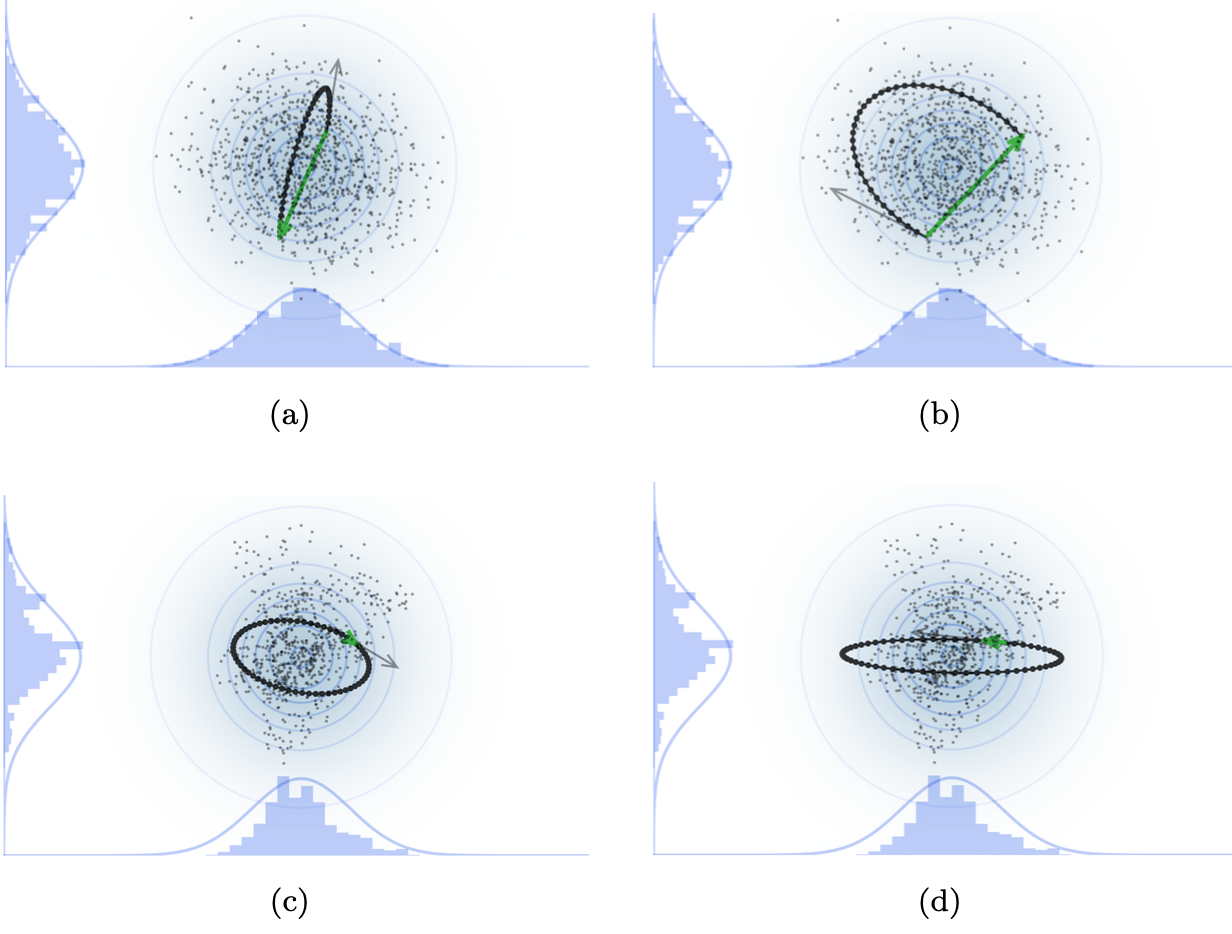
\includegraphics[width=\textwidth]{pics/HMC_Example.png}
    \caption{A simulation example with HMC for a bivariate Gaussian target distribution with $\boldsymbol{\mu}= \begin{bmatrix}
            0 & 0
            \end{bmatrix}$ and covariance matrix
            $\boldsymbol{\Sigma}= 
            \begin{bmatrix}
                1 & 0\\
                0 & 1   
            \end{bmatrix}$. Subfigure (a) and (b) shows a HMC simulation example with a proper choice for $\varepsilon$ and $L$, where the target distribution is thoroughly explored. Subfigure (c) and (d) is the same example, modified with a poor choice of values for $\varepsilon$ and $L$, where the target distribution is poorly approximated. This is especially clear on the plots of the marginal distributions where the histograms are far from the plotted correct distribution. The result is the U-Turn effect, which yield an ineffective exploration of the target distribution. The example has been generated with the interactive gallery provided by \cite{feng} \textcopyright MIT.}
    \label{fig:HMC_Example}
\end{figure}

\begin{algorithm}\label{alg:HMC}
\SetAlgoLined
\SetKwFunction{Leapfrog}{Leapfrog}
\KwInput{An intial parameter $\boldsymbol{\theta}^{(0)}$}
\KwInput{A log-probability distribution $\mathcal{L}$}
\KwInput{Total number of iterations $M$}
\KwInput{Size of leapfrog-steps $\varepsilon$}
\KwInput{Number of leapfrog-steps before generating candidate state, $L$.}
\KwOutput{Set of accepted parameters}

$\text{Given } \boldsymbol{\theta}^{(0)},  \mathcal{L}, M, \varepsilon, L,$\\
\For{m=1,2 \dots, M}{
Sample $\boldsymbol{\rho}^{(0)} \sim \mathcal{N}(0, \boldsymbol{\boldsymbol{I}})$ \\
Set $ \boldsymbol{\theta}^{\text{cand}} \leftarrow \boldsymbol{\theta}^{(m-1)}, \boldsymbol{\rho}^{\text{cand}} \leftarrow \boldsymbol{\rho}^{(0)}$\\
\For{i = 1 to L}{
Set $\boldsymbol{\theta}^{\text{cand}}, \boldsymbol{\rho}^{\text{cand}} \leftarrow \Leapfrog(\boldsymbol{\theta}^{\text{cand}}, \boldsymbol{\rho}^{\text{cand}}, \varepsilon)$
}
Negate momentum: $\boldsymbol{\rho}^{\text{cand}} \leftarrow - \boldsymbol{\rho}^{\text{cand}}$\\
Compute acceptance probability:\\
$\alpha=\min \left\{1, \frac{\exp \left\{\mathcal{L}(\boldsymbol{\theta}^{\text{cand}})-\frac{1}{2} \boldsymbol{\rho}^{\text{(cand)}^\top}  \boldsymbol{\rho}^{\text{cand}}\right\}}{\exp \left\{\mathcal{L}\left(\boldsymbol{\theta}^{(m-1)}\right)-\frac{1}{2} \boldsymbol{\rho}^{(0)^\top}  \boldsymbol{\rho}^{(0)}\right\}}\right\}$\\
Sample $u\sim \text{Uniform}(0,1)$\\
 \uIf{$u<\alpha$}{
    Accept the proposal: $\boldsymbol{\theta}^{(m)} \leftarrow \boldsymbol{\theta}^{c a n d}$\\
  }
  \Else{
    Reject the proposal: $\boldsymbol{\theta}^{(m)} \leftarrow \boldsymbol{\theta}^{(m-1)}$ \\
  }
}
\SetKwProg{Fn}{Function}{:}{\KwRet{$\boldsymbol{\theta}^{\text{cand}},\boldsymbol{\rho}^{\text{cand}}$}}
\Fn{\Leapfrog{$\boldsymbol{\theta}$, $\boldsymbol{\rho}$, $\varepsilon$}}{
 Set $\boldsymbol{\rho}^{\text{cand}} \leftarrow \boldsymbol{\rho}^{\text{cand}}+(\varepsilon / 2) \nabla_{\theta} \mathcal{L}(\theta)$\\
Set $\boldsymbol{\theta}^{\text{cand}} \leftarrow \theta+\varepsilon \boldsymbol{\rho}^{\text{cand}}$\\
Set  $\boldsymbol{\rho}^{\text{cand}} \leftarrow \boldsymbol{\rho}
^{\text{cand}}+(\varepsilon / 2) \nabla_{\theta} \mathcal{L}(\boldsymbol{\theta}^{\text{cand}})$
  }
\caption{Hamiltonian Monte Carlo}
\end{algorithm}




\clearpage
\subsection{No-U-Turn Hamiltonian Monte Carlo}\label{sec:nuts}
In this section we present an algorithm introduced by \cite{hoffman2011nouturn} and evaluated by \cite{nishio_arakawa_nouturn}, whose explanation we found more clear and concise. No-U-Turn (NUTS) extends HMC by eliminating the need to specify the trajectory length $L$. This algorithm gets its name by avoiding the possible U-Turning behavior shown in figure \ref{fig:HMC_Example} (c) and (d). This is done by introducing a criterion that tells us when to stop simulating the dynamics to prevent a possible U-turn. The authors define this criterion to be when performing another leapfrog step will no longer increase the distance between the proposed state $\boldsymbol{\theta}^{\text{cand}}$ and the initial value $\boldsymbol{\theta}^{(0)}$. More specifically, they choose a criterion, based on the derivative with respect to time of half the squared distance between the initial parameter $\boldsymbol{\theta}^{(0)}$ and the current state $\boldsymbol{\theta}^{\text{cand}}$, meaning that leapfrog steps are performed until 
\begin{equation*}
\begin{split}
    \frac{d}{d t} \frac{(\boldsymbol{\theta}^{\text{cand}}-\boldsymbol{\theta})^\top \cdot(\boldsymbol{\theta}^{\text{cand}}-\boldsymbol{\theta})}{2}&=(\boldsymbol{\theta}^{\text{cand}}-\boldsymbol{\theta})^\top \cdot \frac{d}{d t}(\boldsymbol{\theta}^{\text{cand}}-\boldsymbol{\theta})\\
    &=(\boldsymbol{\theta}^{\text{cand}}-\boldsymbol{\theta})^\top \cdot \boldsymbol{\rho}^{\text{cand}} < 0
\end{split}
\end{equation*}
However, \cite{hoffman2011nouturn} notes that by doing this we do not have the guarantee of time reversibility, so the sampling algorithm might not converge to the correct distribution. NUTS overcomes this problem by using slice sampling and applying a double method suggested by \cite{neal_slice_sampling}. 
\\
\\
NUTS augments the distribution of HMC, $p \lr{\boldsymbol{\theta}, \boldsymbol{\rho}} \propto \exp{\left(\mathcal{L} \lr{\boldsymbol{\theta}} - \frac{1}{2} \boldsymbol{\rho}^\top \boldsymbol{\rho}\right)}$, to include a slice variable $u$ so that the joint probability of $\boldsymbol{\theta}, \boldsymbol{\rho}$ and $u$ is 
\begin{equation*}
    p \lr{\boldsymbol{\theta}, \boldsymbol{\rho}, u} \propto \mathbf{1} \lrs{ u \in \lrs{0,\exp{\left(\mathcal{L} \lr{\boldsymbol{\theta}} - \frac{1}{2} \boldsymbol{\rho}^\top \boldsymbol{\rho}\right)}}}
\end{equation*}
meaning that the un-normalized marginal probability of $\boldsymbol{\theta}$ and $\boldsymbol{\rho}$ (gained by integrating over $u$) is 
\begin{equation*}
    p \lr{\boldsymbol{\theta}, \boldsymbol{\rho}} \propto \exp{\left(\mathcal{L} \lr{\boldsymbol{\theta}} - \frac{1}{2} \boldsymbol{\rho}^\top \boldsymbol{\rho}\right)}
\end{equation*}
The conditional probabilities $p \lr{u \mid \boldsymbol{\theta}, \boldsymbol{\rho}}$ and $p \lr{\boldsymbol{\theta}, \boldsymbol{\rho} \mid u}$ are each uniform as long as the condition
\begin{equation} \label{eq:nuts_unif_condition}
    u \leq \exp{\left(\mathcal{L} \lr{\boldsymbol{\theta}} - \frac{1}{2} \boldsymbol{\rho}^\top \boldsymbol{\rho}\right)}
\end{equation}
is satisfied. The challenge of slice sampling is to find the bounds of the region for which this condition is satisfied. \cite{neal_slice_sampling} proposes a doubling method, where the size of the initial segment containing the current value of $\boldsymbol{\theta}$ is randomly chosen and afterwards expanded by doubling its size until the samples are outside of the region. The expanding directions are randomly chosen to be leapfrog steps forward or backward in the Markov chain to satisfy reversibility.
\\
\\
NUTS generates a finite set of all $\lr{\boldsymbol{\theta}, \boldsymbol{\rho}}$ by iteratively doubling its size. The doubling process is stopped to satisfy the condition 
\begin{equation*}
    \lr{\boldsymbol{\theta}^+ - \boldsymbol{\theta}^-}^\top \boldsymbol{\rho}^- < 0 \quad \text{or} \quad \lr{\boldsymbol{\theta}^- - \boldsymbol{\theta}^+}^\top \boldsymbol{\rho}^+ < 0
\end{equation*}
where $\boldsymbol{\theta}^+, \boldsymbol{\rho}^-$ and $\boldsymbol{\theta}^+, \boldsymbol{\rho}^-$ is the leftmost and rightmost variables of all $\lr{\boldsymbol{\theta}, \boldsymbol{\rho}}$ generated by the doubling process respectively. 
\\
\\
A subset of proposal candidates $\lr{\boldsymbol{\theta}, \boldsymbol{\rho}}$, denoted by $\mathbb{C}$, is selected from the doubling process to satisfy the condition in equation \ref{eq:nuts_unif_condition}. The new values of $\lr{\boldsymbol{\theta}^*, \boldsymbol{\rho}^*}$ are then afterwards sampled uniformly from $\mathbb{C}$. 
\\
\\
To further improve this algorithm \cite{hoffman2011nouturn} used the following transition kernel in each step of doubling
\begin{equation*}
\resizebox{\textwidth}{!}{$
T\left(\boldsymbol{\theta}^{*}, \boldsymbol{\rho}^{*} \mid \boldsymbol{\theta},\boldsymbol{\rho}, \mathbb{C}\right)=\begin{cases} \frac{\mathbf{1}\left[\boldsymbol{\theta}^{*}, \boldsymbol{\rho}^{*} \in \mathbb{C}^{\text{new}}\right]}{\left|\mathbb{C}^{\text{new}}\right|} & \text{  when } \left|\mathbb{C}^{\text{new}}\right|>\left|\mathbb{C}^{\text{old}}\right|\\
\frac{\left|\mathbb{C}^{\text{new}}\right|}{\left|\mathbb{C}^{\text{old}}\right|} \frac{\mathbf{1}\left[\boldsymbol{\theta}^{*}, \boldsymbol{\rho}^{*} \in \mathbb{C}^{\text{new}}\right]}{\left|\mathbb{C}^{\text{new}}\right|}+\left(1-\frac{\left|\mathbb{C}^{\text{new}}\right|}{\left|\mathbb{C}^{\text{old}}\right|}\right) \mathbf{1}\left[\left(\boldsymbol{\theta}^{*}, \boldsymbol{\rho}^{*}\right)=(\boldsymbol{\theta}, \boldsymbol{\rho})\right] 
&\text{  when } \left|\mathbb{C}^{\text{new}}\right|\leq\left|\mathbb{C}^{\text{old}}\right|
\end{cases}$
}
\end{equation*}
where $\mathbb{C}^{\text{new}}$ is the subset of $\lr{\boldsymbol{\theta}, \boldsymbol{\rho}}$, added by the last step of the doubling process and $\mathbb{C}^{\text{old}}$ is the disjoint subset of $\mathbb{C}$ so that $\mathbb{C} = \mathbb{C}^{\text{new}} \cup \mathbb{C}^{\text{old}}$. This transition kernel proposes a move from a state in $\mathbb{C}^{\text{old}}$ to a random state in $\mathbb{C}^{\text{new}}$ and accepts this move with probability $\frac{\mathbb{C}^{\text{new}}}{\mathbb{C}^{\text{old}}}$. The authors show that $T$ satisfies the detailed balance condition so that it leaves the uniform distribution over $\mathbb{C}$ invariant. According to \cite{nishio_arakawa_nouturn} this transitional kernel permits memory-efficient implementation and produces larger jumps on average than simple uniform sampling. 
\\
\\
NUTS is especially efficient as it can automatically choose a step size that achieves an acceptance probability around a desired level. The stepsize $\varepsilon$ for the $j$th iteration of a NUTS Markov chain is tuned as follows
\begin{equation*}
    \begin{split}
        \log\lr{\varepsilon_{j+1}} &= \mu - \frac{\sqrt{j}}{\gamma} \frac{1}{j + j_0} \sum_{i=1}^j \lr{\delta - \alpha_i}\\
        \log \lr{\bar{\varepsilon}_{j+1}} &= \eta_j \log \lr{\varepsilon_{j+1}} + \lr{1 - \eta_j} \log \lr{\bar{\varepsilon}_j} \\
        \varepsilon_{j+1} &= \bar{\varepsilon}_{j+1}
    \end{split}
\end{equation*}
where $\alpha_j$ is an actual acceptance probability for the $j$th iteration, $\delta$ is the desired average acceptance probability, $\mu$ is a freely chosen point that the iterated $\varepsilon_j$ shrinks towards, $\gamma$ is a free parameter that controls the shrinkage amount towards $\mu$ and $j_0$ is a free parameter that dampens early exploration. 
\\
\\
\cite{hoffman2011nouturn} introduces the variables $\eta_j = j^{-\kappa}$ with $\kappa < 1$ to give more recent iterates more weight. They show that this way of adapting stepsize guarantees that $\alpha \rightarrow \delta$. They recommend setting $\mu = \log \lr{10 \varepsilon_1}$ and $\delta \approx 0.6$.
\\
\\
NUTS tunes $\varepsilon$ during a predetermined warm-up phase and fixes this value thereafter. Since the algorithm accepts or rejects $\lr{\boldsymbol{\theta}^*, \boldsymbol{\rho}^*}$ from multiple candidates, an alternative statistic to the Metropolis acceptance probability must be defined. They do this by defining for each iteration the acceptance probability by
\begin{equation*}
    \alpha_{j}=\frac{1}{\left|B_{j}\right|} \sum_{\boldsymbol{\theta}, \boldsymbol{\rho} \in B_{j}} \min \left\{1, \frac{p\left(\boldsymbol{\theta}^{j}, \boldsymbol{\rho}^{j}\right)}{p\left(\boldsymbol{\theta}^{j-1}, \boldsymbol{\rho}^{j, 0}\right)}\right\}
\end{equation*}
The pseudocode for NUTS can be seen in algorithm \ref{alg:nuts}.

\begin{algorithm} \label{alg:nuts}
    \SetAlgoLined
    \KwInput{Initial parameters $\boldsymbol{\theta}^{(0)}$}
    \KwInput{A log-probability distribution $\mathcal{L}$}
    \KwInput{Initial size of leapfrog-steps $\bar{\varepsilon_0}$}
    \KwInput{Desired average of acceptance probability $\delta$}
    \KwInput{Aim point for values of the iterated $\varepsilon_j$ values $\mu$}
    \KwInput{Parameter controlling shrinkage towards $\mu$, $\gamma$}
    \KwInput{Parameter that controls dampening of early exploration $j_0$}
    \KwInput{Parameter that controls how much more weight are given to more recent iterates $\kappa < 1$}
    \KwInput{Total number of total number of iterations $J$}
    \KwInput{Total number of iterations for adapting size of leapfrog steps $J^{\text{adapt}}$}
    \KwOutput{Samples from the target distribution}
    \For{j=0, \dots,  J}{
    Sample momentum $\boldsymbol{\rho}^{\text{init}} \sim N(0, \boldsymbol{I})$\\
    Sample auxiliary variable $u \sim \operatorname{Uniform}\left(0, \exp \left(\mathcal{L}\left(\boldsymbol{\theta}^{(j)}\right)-\frac{1}{2}\boldsymbol{\rho}^{\text{init}^{\top}} \boldsymbol{I}^{-1} \boldsymbol{\rho}^{\text{init}}\right)\right)$\\
    Generate $\mathbb{C}$ by using the doubling method with transition kernel $T$. \\
    Compute acceptance probability: $\alpha_{j}=\frac{1}{\left|B_{j}\right|} \sum_{\theta, \boldsymbol{\rho} \in B_{j}} \min \left\{1, \frac{p\left(\boldsymbol{\theta}^{j+1}, \boldsymbol{\rho}^{j+1}\right)}{p\left(\boldsymbol{\theta}^{j}, \boldsymbol{\rho}^{\text{init}}\right)}\right\}$\\
     Accept the proposal $\left(\boldsymbol{\theta}^{*}, \boldsymbol{\rho}^{*}\right)$ with probability $\alpha_{j}$. \\
    \uIf{$j\leq J^{\text{adapt}}$}{
        $\log\lr{\varepsilon_{j+1}} \leftarrow \mu - \frac{\sqrt{j}}{\gamma} \frac{1}{j + j_0} \sum_{i=1}^j \lr{\delta - \alpha_i}$\\
        $\log \lr{\bar{\varepsilon}_{j+1}} \leftarrow j^{-\kappa}\log \lr{\varepsilon_{j+1}} + \lr{1 - j^{-\kappa}} \log \lr{\bar{\varepsilon}_j}$ \\
        $\varepsilon_{j+1} \leftarrow \bar{\varepsilon}_{j+1}$
    }
    \Else{
    $\varepsilon_{j+1}=\varepsilon_{J^{\text{adapt}}}$
    }    
    }
     \caption{No-U-Turn Sampler with Dual Averaging. One can easily change this pseudocode to one that runs until a certain number of samples are collected. For a more detailed pseudocode see \cite{hoffman2011nouturn}.}
\end{algorithm}



\clearpage
\section{Priors}\label{sec:priors}
From section \ref{sec:bayesian_stat} and the example given in section \ref{sec:simple_BNN} it is seen that Bayesian inference starts with a prior for the model parameters, which is supposed to embody ones prior beliefs about the assigned task. The prior is an important component and choosing a bad prior can affect the resulting posterior greatly. That said, the prior does have a diminishing effect on the posterior as the number of samples grow, as the likelihood will concentrate the posterior around a few highly likely parameters. One might think that if one has no qualified prior belief, then a weak prior, like a wide uniform distribution, can be a safe bet, but this can however have various unforeseen consequences as pointed out by \cite{lemoine2019} and \cite{sarma_kay2020}. \\
\\
The prior component is however more than a dangerous element that threatens the quality of the posterior. The prior provides a principled mechanism for researchers to incorporate previous research and knowledge into the model. Priors can also be beneficial in small sample sizes as the prior acts to regularize and reduce the chances of overfitting.
Although in neural networks the relationship between parameters and the problem can be very abstract and not as intuitive as in other machine learning models like linear regression models or support vector machines, so having qualified prior beliefs about the weights might not be so easy. 
\\
\\
\cite{neal2012bayesian} stresses that even though it can seem like BNNs can be threatened by a lack of a suitable prior this is not the case, as much past work shows useful criteria for selecting suitable priors, even without full understanding of what the prior over the parameters will mean in terms of the output of the network. \cite{mackay1991} and \cite{MacKay1992} has produced results, that \cite{neal2012bayesian} describes as at least reasonable, by giving the parameters Gaussian prior distributions. He lets the standard deviation of these distributions be selected as a hyperparameter, which allows the model to adapt to the data. 
\\
\\
According to \cite{neal2012bayesian}, our prior knowledge will often be too unspecific to fix the parameter values chosen for the prior distribution, even if we have complete insight into their effects on the prior. We may then wish to treat these values as unknown hyperparameters, giving them a higher-level broad prior distribution, which we call a hyper-prior. \cite{neal2012bayesian} refers to these as Hierarchical models. One benefit of such models is that the appropriate degree of regularization for the task can be determined automatically from the data, see \cite{mackay1991} and \cite{MacKay1992}. 







